\chapter{Cascaded Subpatch Networks for Effective CNNs}

{\small \textbf{Authors}\\
Xiaoheng Jiang, Yanwei Pang, \textit{Senior Member, IEEE}, Manli Sun, and Xuelong Li, \textit{Fellow, IEEE}\\ \\
IEEE TRANSACTIONS ON NEURAL NETWORKS AND LEARNING SYSTEMS\\VOL. 29, NO. 7, JULY 2018}

\section{Proposed Method}

In this first paper we are going to talk about a new way to perform the convolution operation. It has been noted that the classical convolution might not be as efficient as we might think. As we know, the convolution is usually performed as an element-wise multiplication between an input patch of the image and a filter of a fixed size $H \times W$. Here, the novel approach is to represent the filter used for the convolution through subpatches that have a smaller size than the original filter. Basically, rather than convolving one filter with the input image, we will go through a gradual decrease of the filter size until it becomes of size $1 \times 1$. In order to do so, each subpatch will be made of two filters. The first one will represent the spatial size $h \times w$, while the second one will be the scalar result of size $1 \times 1$. It is noted that the size of a subpatch is always smaller than its previous. For instance, if the original patch is $H \times W$, the first subpatch must be such that $H > h$ and $W > w$ and so on. The idea is to convolve the subpatch filter with the input patch and then, by taking the output of this operation we feed it through another patch until we end up having just one neuron. Doing so, we represent these cascaded subpatches through a pyramid. It is worth to show the difference between a classical convolution and the one proposed here. In Figure \ref{fig:01_1}, the classical convolution returns a scalar value. On the other hand, in Figure \ref{fig:01_2}, we start with a patch of size $H \times W$ and we wind up with a single neuron. In this way, a \textit{csconv} filter is created and it basically represents just one filter. If many of these csconv filters are stacked layer by layer, a CSNet is created.

\begin{figure}[h!]
    \centering
    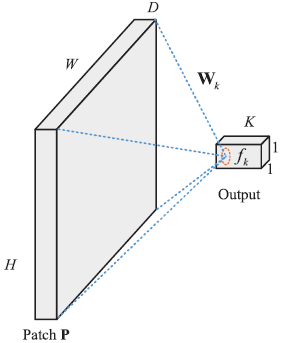
\includegraphics[scale=0.6]{images/01_1.png}
    \caption{Conventional convolutional filter}
    \label{fig:01_1}
\end{figure}

\FloatBarrier

\begin{figure}[h!]
    \centering
    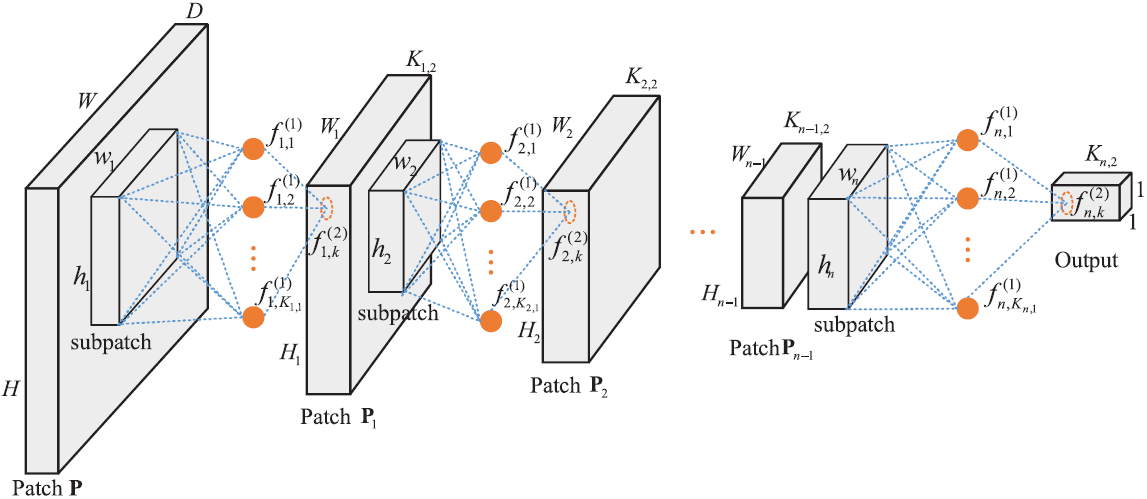
\includegraphics[scale=0.50]{images/01_2.png}
    \caption{n-stage \textit{csconv} filter $[(h_1 \times w_1, 1 \times 1), (h_2 \times w_2, 1 \times 1), ..., (h_n \times w_n, 1 \times 1)]$}
    \label{fig:01_2}
\end{figure}

\FloatBarrier

\section{Experimental Results}

In this section, experimental results are evaluated. First of all let us say that the proposed method has been evaluated on a few datasets. The datasets considered are: CIFAR10 \citep{CIFAR10and100}, CIFAR100 \citep{CIFAR10and100}, MNIST \citep{MNIST}, street view house numbers (SVHN) \citep{SVHN} and ImageNet 2012 \citep{ImageNet12}. Moreover, three different architectures of the CSNet have been used. The main difference among them is the number of the parameters, which is lower in the smallest architecture and it is progressively increased in the other two. Anyhow, it is worth mentioning the overall structure of these networks (Figure \ref{fig:01_3}). They are made of $n$ CSconv layers among which some max pooling layers have been added. The pooling operation has not been discussed in great detail yet, but it will be widely explained in another paper. Finally there is a softmax function whose aim is to return the class scores. As far as some of the tecniques employed in this work, we mention dropout, batch normalization and weight decay. Their purpose is basically to control overfitting and reduce the number of parameters. By testing this model on the mentioned datasets, very good results are obtained. This is translated into a real effectiveness of the cascaded subpatches method.\\

\begin{figure}[h!]
    \centering
    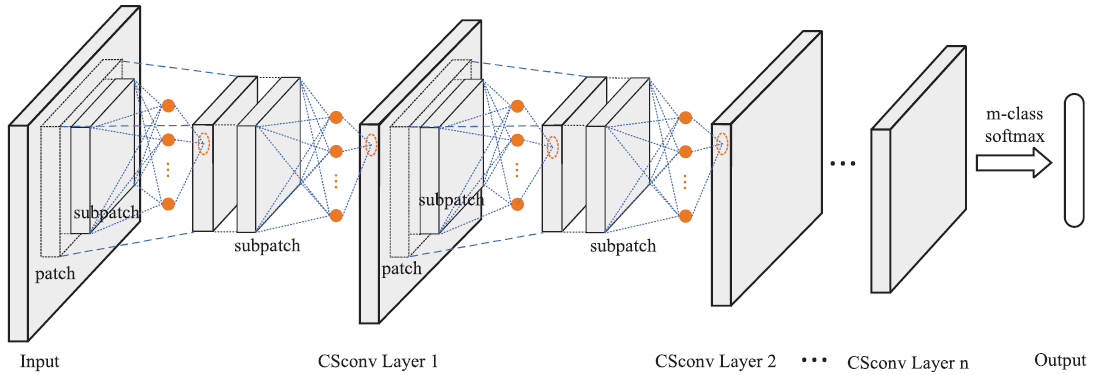
\includegraphics[scale=0.52]{images/01_3.png}
    \caption{Overall structure of CSNet}
    \label{fig:01_3}
\end{figure}

\FloatBarrier